\section{Analisi dei contesti semantici di un sognatore}\label{sec:analisi-dei-contesti-semantici-di-un-sognatore}

In questa sezione verrà esplorato un caso di studio, risultato del tentativo di usare il modello dei grafi multi-livello
allo scopo di individuare dei contesti di parole di valenza sintattica e semantica all'interno del mondo onirico
di una particolare sognatrice, i cui sogni sono stati prelevati dal dataset di sogni di DreamBank.net disponibile
online.
Daremo forma allo spazio delle parole di Emma a partire da un vasto corpus di racconti di sogni, e analizzeremo la
struttura del grafo multi-livello risultante.

\subsection{Pre-elaborazione con strumenti di NLP}

Per poter procedere con l'analisi dei sogni di Emma affinché si potesse costruire un grafo delle parole
da cui poter cogliere aspetti semantici, si è ritenuto necessario aggiungere dei passaggi ulteriori
al processo di pre-elaborazione descritto nella sottosezione~\ref{subec:pre-elaborazione-con-NLP}.
In particolare, si è rivelato utile allo scopo di un'analisi semantica,
un filtraggio delle parole meno frequenti rispetto all'intero corpus di sogni di Emma.
Questo passaggio è stato eseguito per ridurre la complessità del testo e concentrare l'analisi sui
termini più rilevanti e significativi, con l'obiettivo di individuare le tematiche principali trattate
nei sogni e l'ordine con cui esse appaiono nei testi.
Un'altra possibile interessante fase di pre-elaborazione ulteriore è quella dell'estrapolazione di categorie
specifiche di parole.
Attraverso tecniche di NLP come il Part-of-Speech (POS) tagging, ciascuna parola può essere etichettata con la sua
categoria grammaticale di appartenenza, come quella dei sostantivi, verbi, aggettivi, avverbi, ecc.
Con la tecnica di Named Entity Recognition (NER) tagging è possibile, invece, identificare le entità di interesse
all'interno del testo, categorizzando elementi come persone, luoghi e organizzazioni.
A partire da queste categorizzazioni, tutte le parole che non sono etichettate in una particolare
categoria vengono filtrate. Lo scopo di questa fase potrebbe essere quello di concentrare l'analisi sulle parole che
sono considerate le parti del testo più significative e ricche di contenuto, o semplicemente focalizzare l'analisi
su un aspetto di interesse.


\subsection{Riduzione della connettività del grafo delle parole}\label{subsec:elaborazione-del-grafo-delle-parole}

Sebbene il grafo delle parole risultante dalla pre-elaborazione di tutti i sogni di un particolare sognatore
sia frutto di un processo di semplificazione e riduzione della complessità del testo, la sua analisi diretta
attraverso l'uso del grafo multi-livello ne ha rivelato sin da subito la sua elevata connettività derivante dalla
natura del linguaggio naturale: parole e concetti possono essere strettamente legati (e quindi ``vicini'') ad un
ampio numero di altri concetti che a loro volta possono collegarsi direttamente ad altri concetti sparsi per il grafo.
Il risultato è uno spazio fortemente ``aggrovigliato'' che non favorisce la formazione di gruppi di parole distinti e
ben definiti e che, di conseguenza, non favorisce un processo di contrazione di qualità nella
gerarchia del grafo multi-livello.

Per rendere chiaro questo aspetto, si prenda come esempio il grafo multi-livello $M = (G, \langle f_{C_1}, f_{C_2}\rangle)$
rappresentato in figura~\ref{fig:les-miserables-graph}, il cui grafo $G$ rappresenta il grafo delle relazioni di
co-apparizione dei personaggi del romanzo \textit{Les Misérables} di Victor Hugo,
e le cui funzioni di contrazione $f_{C_1}$ e $f_{C_2}$ rappresentano rispettivamente le funzioni di contrazione
per cricche non reciproche e stelle.
Appare evidente di come la struttura del grafo $G$ sia stata contratta con un elevato tasso di contrazione,
producendo una struttura notevolmente più semplice e facilmente interpretabile. Per via degli schemi di
contrazione scelti, appare evidente come la struttura originale del grafo abbia rivelato la sua ordinatezza ai livelli
superiori: in media i personaggi del romanzo possono apparire assieme ad una cerchia ristretta di altri personaggi,
ad eccezione di personaggi principali che risultano collegarsi a questi gruppi più o meno isolati di nodi.
Questo rispecchia in parte la natura dello spazio bidimensionale in cui i personaggi sono collocati: personaggi
appartenenti a luoghi distanti difficilmente appariranno insieme. I personaggi principali, in quanto seguiti
nella narrazione nel mentre che si spostano nello spazio, permettono di rompere questa dimensionalità, e risultano
essere collegati a nodi distanti tra loro.

\begin{figure}[h]
    \centering
    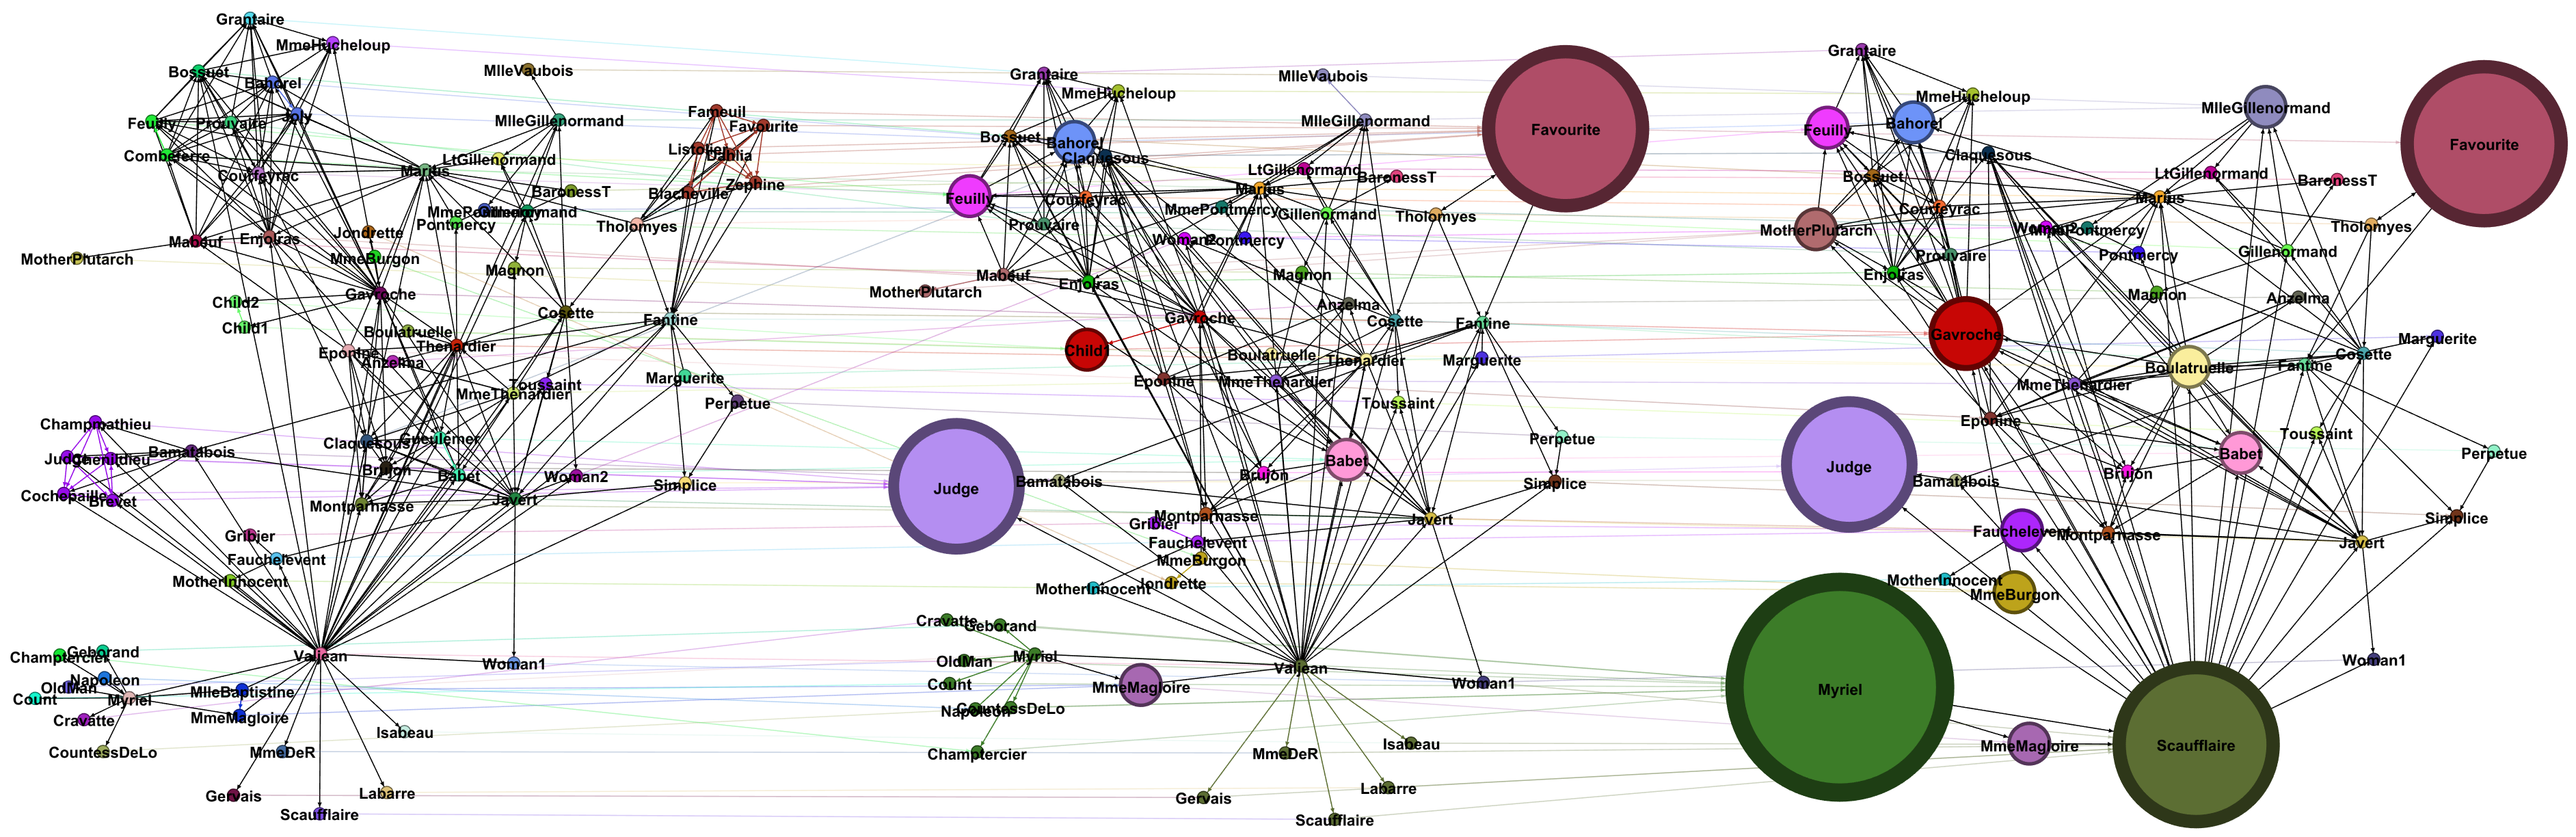
\includegraphics[width=0.8\textwidth]{Immagini/les_miserables_example.png}
    \caption{Grafo multi-livello delle co-apparizioni in \textit{Les Misérables}}
    \label{fig:les-miserables-graph}
\end{figure}

Per risolvere questo problema legato all'alta connettività del grafo delle parole, si è deciso di applicare
una tecnica di potatura del grafo, che consiste nell'identificazione di uno scheletro portante del grafo
basato sulle relazioni più significative tra le parole e dell'esclusione delle relazioni meno significative in
accordo a tale scheletro, allo scopo di ``appiattire'' lo spazio delle parole.

\nlparagraph{Classificazione degli archi}

L'algoritmo di potatura del grafo si basa sulla rilevanza delle relazioni tra le parole, ovvero degli archi del grafo.
Sebbene la rilevanza di un bigramma possa essere definita e valutata in diversi modi - come ad esempio il calcolo
dell'informazione mutua puntuale (PMI) tra le parole - in questo caso si è scelto di basare la rilevanza
direttamente sull'informazione fornita dai pesi degli archi e dei relativi nodi coinvolti.
In particolare, la misura di rilevanza di un arco è stata definita come la somma dei rapporti tra il peso dell'arco
e i singoli pesi dei nodi su cui l'arco è incidente.
In formule, siano $w(u)$, $w(v)$ e $w(u, v)$ il peso del nodo $u$ e $v$ e dell'arco $(u, v)$ rispettivamente,
la rilevanza dell'arco $(u, v)$ è definita come:
\begin{equation*}
    relevance(u, v) = \frac{w(u, v)}{w(u)} + \frac{w(u, v)}{w(v)}
\end{equation*}

La formula fornisce un criterio elementare per distinguere la frequenza di coppie di parole dalla loro importanza:
un arco con un peso elevato rispetto ai pesi dei nodi coinvolti è considerato più rilevante di un arco con un peso
elevato rispetto alla media dei pesi degli altri archi.
Ad esempio, un arco con peso 10 tra due nodi con pesi 100 e 200 è considerato meno rilevante di un arco con peso 5
tra due nodi con pesi 8 e 10. \newline

La scelta di questa misura di rilevanza è dovuta alla facilità con cui è possibile associarla ad un nuovo valore
positivo che rappresenti una distanza semantica tra le parole collegate.
Essendo tale valore di rilevanza sempre compreso nell'intervallo $(0, 2]$, è possibile definire un valore di costo
semantico dell'arco $(u, v)$ come $\frac{1}{relevance(u, v)}$, che è inversamente proporzionale alla
rilevanza dell'arco.
Gli archi possono, quindi, essere classificati in base a questo valore di distanza che d'ora in avanti chiameremo
\textit{costo} dell'arco.

\nlparagraph{Algoritmo per la riduzione della connettività}

Un algoritmo che sfrutti l'informazione data dal costo degli archi per ridurre la complessità e la connettività
di un grafo potrebbe agire costruendo in maniera incrementale un nuovo grafo a partire da quello fornito in input,
che ne rappresenti una versione semplificata.
L'algoritmo proposto nel seguente pseudocodice considera gli archi del grafo in input $G$ in ordine crescente di
costo al fine di valutarne l'inclusione nel nuovo grafo semplificato $H$, sulla base di un ulteriore parametro in input
che chiamiamo \textit{threshold}.

In particolare, ogni nodo del grafo originale $G$ sarà presente nel grafo semplificato $H$. Mentre per ogni arco $(u, v)$
di $G$ considerato nel ciclo for a riga 4, se nella versione non orientata di $H$, ottenuta rimuovendo l'orientamento
degli archi, esiste già un cammino tra i nodi $u$ e $v$ e il costo del cammino minimo calcolato sul costo degli archi
è maggiore al threshold, l'arco $(u, v)$ viene ignorato, altrimenti viene aggiunto al grafo semplificato $H$.
Si noti che nello pseudocodice, così come nella notazione tipica, un costo di cammino minimo pari a $\infty$ indica
che non esiste un cammino tra i nodi.

\begin{algorithm}[H]
    \caption{REDUCE-CONNECTIVITY($G$, $threshold$)}\label{alg:reduce-connectivity}
    \begin{algorithmic}[1]
        \State Sia $H = (W, F)$ un nuovo grafo orientato, con $W = G.V$ e $F = \emptyset$
        \State Sia $H_u = (W_u, F_u)$ un nuovo grafo non orientato, con $W_u = G.V$ e $F_u = \emptyset$
        \State Ordina gli archi in $G.E$ in ordine crescente di costo
        \For {$(u, v) \in G.E$}
            \State Sia $d$ il costo del cammino minimo tra $u$ e $v$ in $H_u$ calcolato sulla base del costo degli archi
            \If{$d == \infty$ \textbf{or} $d < threshold$}
                \State $F = F \cup \{(u, v)\}$
                \State $F_u = F_u \cup \{\{u, v\}\}$ \Comment{L'arco aggiunto ha lo stesso costo di $(u, v)$}
            \EndIf
        \EndFor
        \State \textbf{return} $H$
    \end{algorithmic}
\end{algorithm}

In questo modo, l'algoritmo costruisce arco dopo arco un grafo semplificato $H$ basato sui collegamenti più
rilevanti tra le parole.
Gli archi che vengono ignorati sono quelli che collegano parole considerate distanti secondo i collegamenti più
rilevanti stabiliti nello scheletro provvisorio del grafo $H$.
Il grado di tolleranza alla distanza tra le parole è regolato dal parametro \textit{threshold},
che può essere impostato per ottenere un grafo più o meno semplificato: più basso sarà il threshold, minore
sarà il grado di connettività del grafo prodotto.

\nlparagraph{Complessità}
Il costo dell'algoritmo REDUCE-CONNECTIVITY è principalmente dominato dalla fase di ordinamento degli archi
e del calcolo dei cammini minimi tra i nodi del grafo non orientato $H_u$.
Utilizzando algoritmi di ordinamento efficienti, il costo computazionale dell'ordinamento a riga 3 è $O(|E| \log |E|)$.
Il calcolo dei cammini minimi tra i nodi di $H_u$ a riga 5 può essere eseguito in tempo $O(|V| \log{|V|} + |E|))$
utilizzando l'algoritmo di Dijkstra con coda di priorità gestita da heap di Fibonacci.
Essendo che il ciclo for a riga 4 viene eseguito una volta per ogni arco in $|E|$, il costo totale dell'algoritmo
risulta essere:
\begin{equation*}
      O(|E| \log |E|) + O(|E| \cdot (|V| \log{|V|} + |E|)) \quad = \quad
      O(|E| (\log |E| + |V| \log{|V|} + |E|))
\end{equation*}

\subsection{Analisi dei risultati}\label{subsec:analisi-del-grafo-multi-livello}

Discutiamo ora brevementeil grafo multi-livello dell'intero corpus di 1221 sogni di Emma mostrato in
figura~\ref{fig:mlg-emma-example}, risultante dall'applicazione delle procedure di pre-elaborazione e dalla riduzione
della connettività con un parametro di threshold pari a $11.0$.
Esso è stato ottenuto selezionando i primi 300 lemmi univoci più frequenti, filtrando per categorie POS mantenendo
sostantivi e verbi.
Le funzioni di contrazione applicate sono, in ordine, la contrazione per circuiti semplici,
per componenti fortemente connesse e per stelle, la cui ultima è stata applicata ripetutamente per
formare i cinque livelli più alti.
Ogni nodo al livello $0$ rappresenta un unigramma, con un'etichetta che ne indica il lemma originale. L'etichetta di
supernodi appartenenti al livello $1$ e superiori rappresentano invece l'etichetta del nodo più pesante del livello
precedente tra quelli contratti per formare il supernodo, considerato quindi come rappresentante del gruppo di nodi.
La dimensione di un nodo è infatti proporzionale al suo peso che, al livello $0$, è dato dal numero di occorrenze del
lemma nel corpus di sogni, mentre ai livelli superiori è dato dalla somma dei pesi dei nodi del livello precedente che
sono stati contratti per formare tale supernodo.
Come si può meglio notare dal riquadro ingrandito, nodi dello stesso livello che vengono contratti nello stesso
supernodo assumono un colore uguale, e la relazione nodo-supernodo è indicata da un arco orientato
semi-trasparente dello stesso colore.
Ciò che appare subito evidente è l'elevata complessità della struttura dei grafi ai livelli più bassi, che
via via si semplifica riducendo il numero di nodi e archi ai livelli superiori, ottenendo nodi che accumulano
sempre più peso.

Il rilevamento dei cicli, che identifica sequenze rilevanti di parole che riportano alla parola iniziale, potrebbero
rappresentare schemi influenti o temi ricorrenti nelle narrazioni dei sogni,
potenzialmente indicando collegamenti di pensiero persistenti nei sogni di Emma.
Si noti tuttavia che per l'elevato numero di sogni considerati e per la conseguente scelta del parametro di threshold,
la presenza di cicli è limitata a poche brevi sequenze di parole particolarmente correlate, date da gruppi di
parole come ``cake''- `party, ''boat''-``lake''-``water'', ``trip''-``train''-``station'' oppure
''road''-``car''-``drive''-``hill''.
\'E interessante supporre di come queste sequenze possano fornire delle informazioni rilevanti proprio per via del forte
legame semantico che esse rappresentano.
Ad esempio la sequenza ``liturgy''-``church'-``music'' potrebbe indicare che per Emma il tema della musica è
fortemente associato al contesto della chiesa e alla liturgia, rispetto ad altri contesti che potrebbero
essere maggiormente attinenti per altre persone, come quello di un concerto o di un'accademia musicale.


L'individuazione delle componenti fortemente connesse al livello successivo potrebbe indicare unità tematiche coerenti
che, nel complesso delle narrazioni dei sogni, si co-occorrono e si interconnettono frequentemente tra loro rendendosi
mutualmente raggiungibili.
Queste componenti potrebbero rappresentare cluster di concetti o temi strettamente
interrelati che frequentemente co-occorrono e si interconnettono tra più sogni.
Come si può dedurre confrontando le dimensioni dei nodi al livello $2$ rispetto a quelle del livello precedente,
l'applicazione della contrazione per componenti fortemente connesse, in genere permette di individuare contesti
semanticamente più ampi di quelli visti per la contrazione per circuiti semplici.
Questo è dovuto da un lato alla natura delle componenti stesse, da un altro al fatto che la contrazione avviene
già ad un livello di astrazione superiore, in cui concetti strettamente collegati sono già stati raggruppati in unici
supernodi.
Esempi di insiemi di lemmi originali contenuti in componenti fortemente connesse individuate sono
``sit''-``chair''-``front''-``porch''-``seat''-``plane''
oppure ``lake''-``boat''-``water''-``rise''-``pool''-``swim''-``rush'', che racchiude uno dei circuiti semplici visti
in precedenza.

La contrazione per stelle, infine, permette di inglobare ulteriormente dei supernodi periferici ai quelli principali già
affermati nei primi livelli.
In questo modo lemmi e contesti che ``orbitano'' attorno ad altri e che, quindi,
ne siano strettamente dipendenti, vengono contratti in contesti più generali, espandendosi di una singola unità
di distanza di un arco ad ogni successivo livello.
Lo scopo di queste contrazioni altro non è che quello di far nascere dei macro-cluster che includano la maggior parte
delle parole originali, in maniera simile a come accade per alcuni strumenti di NLP, come i modelli di
\textit{word embedding}, le tecniche di \textit{topic modeling} e algoritmi di clustering semantico.

\begin{figure}[h]
    \centering
    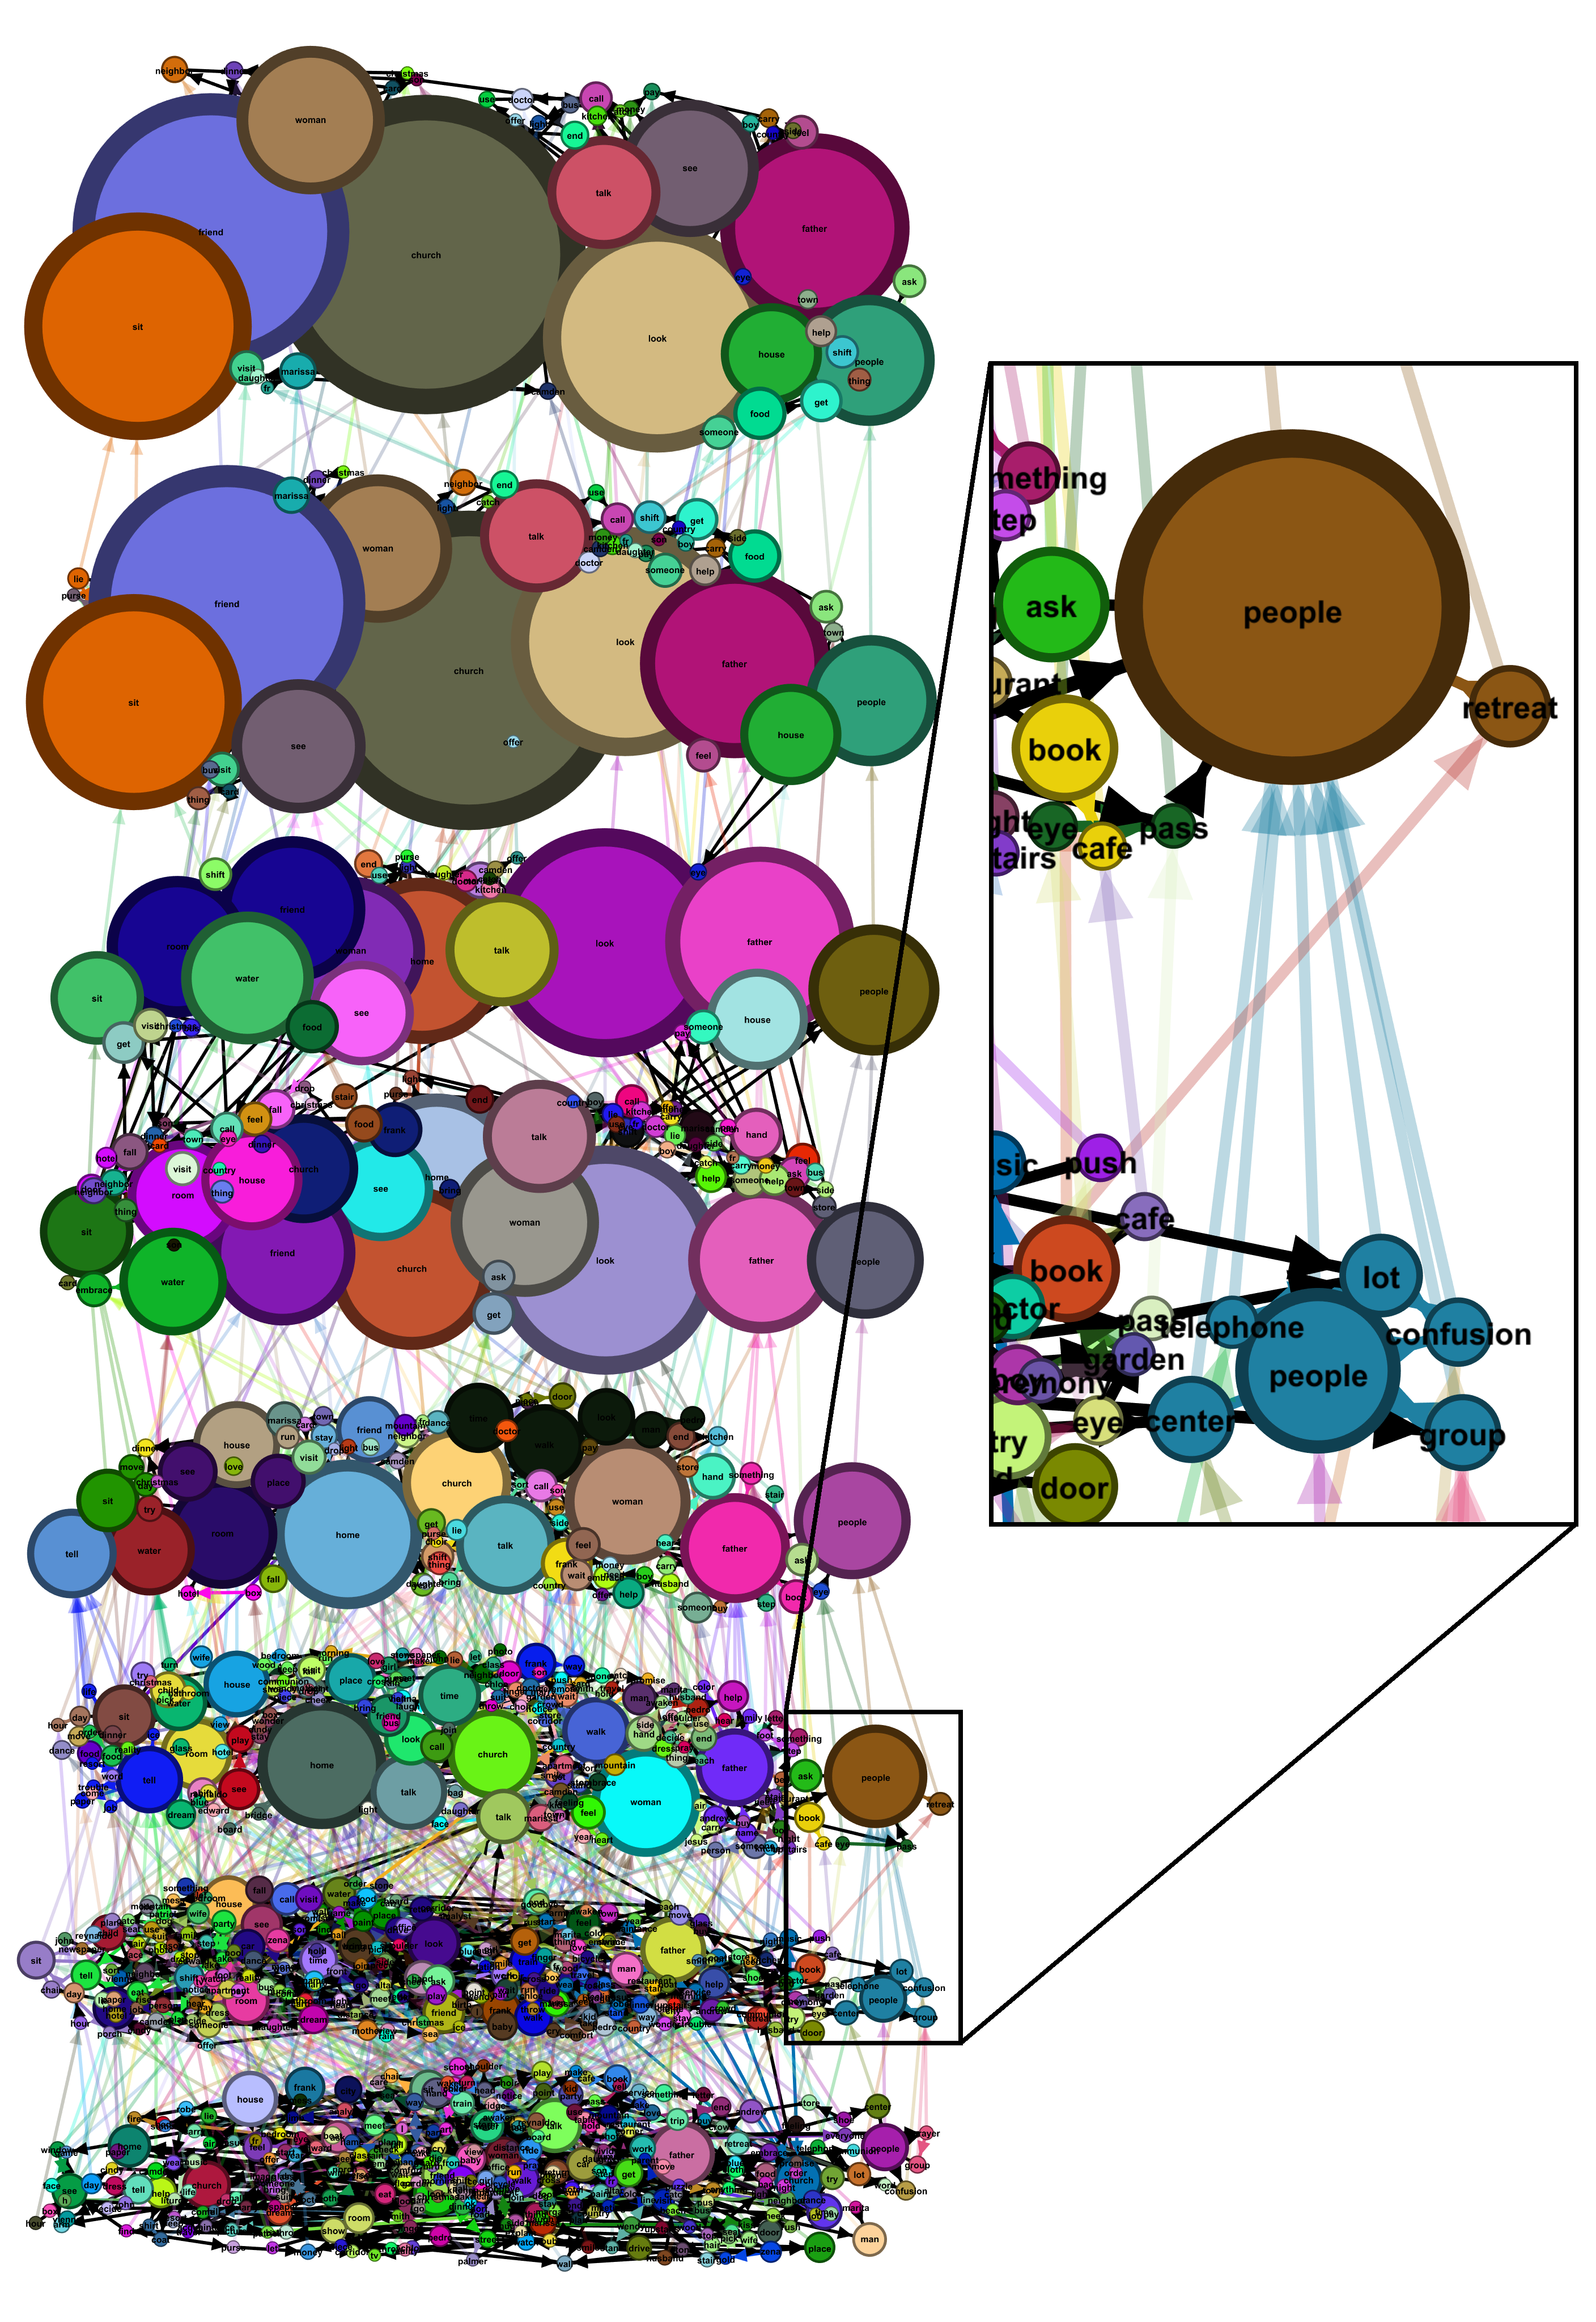
\includegraphics[width=0.8\textwidth]{Immagini/mlg_emma_focus_example.png}
    \caption{Grafo multi-livello del corpus di sogni di Emma}
    \label{fig:mlg-emma-example}
\end{figure}